\chapter{Sparse Transformations}\label{chap:SparseRAJA}

Performance portability libraries (PPLs) are so useful because their abstractions let developers port applications to new systems without rewriting large portions of their code.
Because the abstractions in these libraries are so general, as broad as ``loops and data,'' programmers can use them to represent entire programs portably.
But there is a caveat. 
They can represent entire programs portably, as long as the program does not include any sparse computation where it does not make sense to use a full multidimensional array.
Of course, sparse computations are not so unique that they cannot be written with ``loops and data.''
Rather, writing sparse codes with PPLs often requires sacrificing their portability.
This is because sparse codes work with data stored in a wide range of formats, each with a different interface.
Thus, a code written for one format cannot be used for another without changing significant parts of the code.
Because sparse computations play such a significant role in high-performance computing, representing them portably would be a valuable capability for PPLs\@.
This chapter explores that possibility.
I develop a prototype implementation in RAJA of a format-independent interface for writing sparse computations based on the library's approach to writing dense codes.
While intuitive, the runtime overhead caused by the modifications are too costly.
Ultimately, RAJA's decoupled abstractions (and analogues in other PPLs) for iteration space, schedule, and data access work well for dense codes, but fail to represent the stronger interrelation of data and schedule in sparse codes.
I conclude that the decoupling of data and loop abstractions in PPLs must be relaxed to most effectively support sparse computations and provide some possible approaches to do so based on interfaces targeted by a sparse computation code generator called TACO\@.


\section{Sparse Computations And Data}

%Sparse computations are important.
Sparse computations --- those that operate on data where ``there is advantage to be taken of the percentage or distribution of zero elements''~\cite{duff1977survey} --- have long been a bottleneck for high performance computing applications. 
Even as early as 1971, scientists lamented the difficulty of computing with sparse data~\cite{willoughby1971sparse}.
More than fifty years later, new application domains for sparse computations have garnered attention, including recommendation systems~\cite{he2016fusing} and machine learning~\cite{zhao2018bridging,zhu2019sparse}, and programming sparse applications remains a challenge.
Many of these difficulties emerge from the variety of compression strategies used to avoid storing and computing on zero elements.


\begin{figure*}
  \centering
  \begin{subfigure}{0.45\textwidth}
    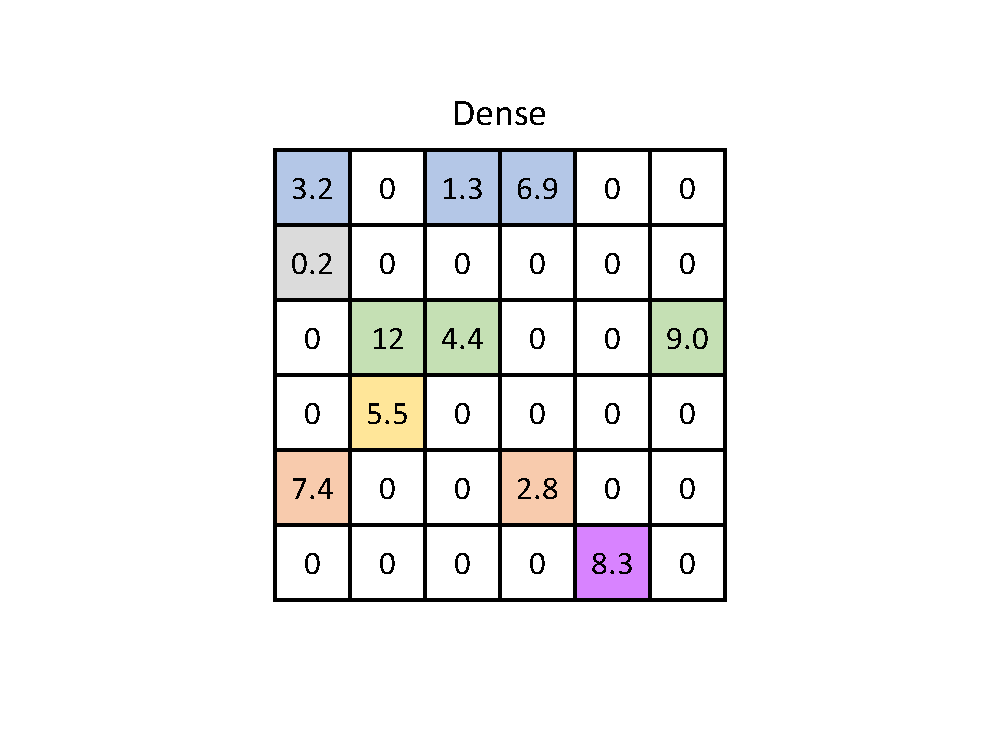
\includegraphics[page=1,width=\textwidth]{FormatDiagram.pdf}
    \caption{Dense representation of data. All entries are stored, including zeros.}\label{FormatDiagram:Dense}
  \end{subfigure}
  \begin{subfigure}{0.45\textwidth}
    \includegraphics[page=2,width=0.95\textwidth]{FormatDiagram.pdf}
    \caption{Coordinate storage (COO) representation of data. The nonzero entries and their corresponding index values are stored. Here, the entries are sorted by row index then by column index.}\label{FormatDiagram:COO}
  \end{subfigure}

  \begin{subfigure}[c]{0.45\textwidth}
    \includegraphics[page=3,width=0.95\textwidth]{FormatDiagram.pdf}
    \caption{Compressed sparse row (CSR) representation of data. Instead of storing duplicate row values, the row array is compressed to the offsets in the column and value arrays where each row starts.}\label{FormatDiagram:CSR}
  \end{subfigure}
\caption{Dense, COO, and CSR storage representations of the same data.  Nonzero entries are colored by their row value.}\label{FormatDiagram}
\end{figure*}
\begin{figure}
  \begin{lstlisting}[caption={Sparse matrix vector multiply (SpMV) routines for matrices in different formats. Note that essentially every line of code is different in each implementation, even though they implement the same computation.},label=DenseAndSparseMV]  
  //Dense
  void dense_matrix_vector_multiply(View2D A, View1D x, View1D y) {
    int Ni = A.num_rows();
    int Nj = A.num_cols();
    for(int i = 0; i < Ni; i++) {
      for (int j = 0; j < Nj; j++) {
        y(i) += A(i,j) * x(j);
      }
    }
  }
  
  //Coordinate storage
  void COO_matrix_vector_multiply(COOView2D A, View1D x, View1D y) {
    int nnz = A.numNonZeros();
    for(int idx = 0; idx < nnz; idx++) {
      int i = A.rows(idx);
      int j = A.cols(idx);
      y(i) += A.vals(idx) * x(j);
    }
  }
  
  //Compressed Sparse Row
  void CSR_matrix_vector_multiply(CSRView2D A, View1D x, View1D y) {
    int Ni = A.numRows();
    for(int i = 0; i < Ni; i++) {
      startIndex = A.rowptr(i);
      endIndex = A.rowptr(i+1);
      for(int j = startIndex; j < endIndex; j++) {
        y(i) += A.vals(j) * x(A.col(j));
      }
    }
  }
  \end{lstlisting}
  \end{figure}
%We need to be able to change sparse data formats,
Like with dense codes, it is often desirable to change the sparse data format a computation uses.
Because of their compression strategies, sparse data structures usually do not support constant-time random access.
Instead, format and schedule are coordinated so that the sparse data is traversed in order, replacing random access with incremental updates to avoid searches and only compute on nonzero entries.
This means that in addition to improving memory performance, a good choice of format can improve the algorithmic complexity of a program.
Changes in algorithm, schedule, machine, and input data all influence which format is best (see Section~\ref{sec:SparseFormats}).
For performance portability, programmers should be able to easily change sparse data format without rewriting entire loop nests.


%and changing sparse formats in handwritten code is more difficult than with dense.
However, portable sparse performance comes at the cost of more significant refactoring.
With handwritten codes, changing the sparse format used in a loop nest can involve changes to every single line of code for the loop nest.
An example of this phenomenon is shown in Listing~\ref{DenseAndSparseMV}, which contains implementations of sparse matrix vector multiplication (SpMV), a key building block for sparse algorithms and a popular evaluation benchmark~\cite{bell2009implementing,buluc2009parallel,liu2013efficient,langr2015evaluation}, for three different formats.
This effect, already present with a simple kernel and commonplace formats, is amplified as the complexity of the loop nest and format increase.
With dense data, no matter the layout, there is a closed form, $O(1)$ complexity function for calculating the location of any element (i.e., typical multidimensional array addressing arithmetic).
The problem: with sparse formats, there is no constant-time random access.
Instead, the loops must be reorganized to stream through the sparse data, even if it means indirect accesses into dense data.
Because the computation is written around streaming through sparse data, most of the code ends up implementing the traversal of the nonzeros rather than the computation the programmer wants to express.


  
%There isn't a performance portable way in RAJA to change sparse formats.
In RAJA, while there is some support for representing sparse computations, there is not a performance portable way to change sparse formats.
The \verb.ListSegment. abstraction can be used to iterate over the coordinates of a sparse structures nonzero entries, but requires the loop nest to be flattened to a one-dimensional traversal.
For a perfectly nested, reorderable computation like SpMV, this is a manageable requirement.
For a computation with dependences and imperfect nesting, like Gauss-Seidel iterative solve, this requirement becomes much more troublesome.
Even after wrangling a computation into this representation, changing the format of the sparse data can mean modifying large swaths of code, both within the computation itself and in constructing its iteration space.

%Ideally, performance portable sparse format changes would enable computations to access data using the same interface regardless of data format.
%RAJA's existing multidimensional data interface is a convenient and intuitive target.
Ideally, performance portable sparse format changes would enable computations to access data using the same interface regardless of data format and layout: dense or sparse.
The existing multidimensional data interfaces in PPLs are a convenient and intuitive target.
With this approach, the description of a sparse computation would look quite similar to a dense version.
In a similar vein, PPLs already contain interfaces for representing a computation's schedule.
If support for sparse computations could be built using these existing abstractions, it would create significant programmability benefits.
The computation would be sparse, but it would look as if it were dense.
 
%Conforming to this interface presents two challenges: traversing the iteration space and traversing the data.
This chapter details the design decisions and lessons learned while developing a prototype of this approach in the RAJA performance portability library.
Conforming to the existing interface of RAJA computations presents two challenges: constructing the iteration space and traversing the sparse data.
I enable iteration space construction by introducing new \verb.SparseSegment. abstractions.
I enable data traversal by incorporating incremental updates into the sparse View's access function.
The prototype supports three classes of formats: permuted coordinate storage, permuted compressed sparse row (compressed sparse column is one permutation), and a coordinate storage format that stores diagonal entries separately.

Given that they have the same algorithmic complexity, I hypothesize an implementation of this approach could compete with one specialized for specific formats.
However, evaluation disproves this hypothesis, showing the increased constant factor incurred by runtime overhead is too expensive, causing a $2-3.5\times$ slowdown.
More aggressive optimization of the approach would come at the cost of restricting the class of sparse computations the approach could represent.
I conclude that approach to decoupling data, iteration space, and schedule in PPLs is sufficient for dense codes, but it cannot represent the more significant coupling of these elements present in sparse codes.
I show how the decoupling between loop abstractions and data access abstractions cause the performance overhead and make suggestions for introducing sparse loop and data abstractions similar to those that have been shown to work in the context of generating efficient sparse tensor code~\cite{kjolstad2017tensor}. 

The rest of this chapter proceeds as follows.
Section~\ref{sec:SparseFormats} reviews the wide variety of sparse formats that have been developed and motivates the need to have the one codebase support multiple sparse formats.
Section~\ref{sec:IndexSets} reviews RAJA's existing capabilities for representing sparse computations and their limitations.
Section~\ref{sec:SparseRAJA} describes the design and implementation of a prototype extension to support format-independent computation descriptions in RAJA\@.
Section~\ref{sec:SparseEval} evaluates the prototype, and Section~\ref{sec:SparseDiscussion} discusses lessons learned and concludes.



\section{A Preponderance of Sparse Data Formats}\label{sec:SparseFormats}

%Key points:
%There are lots and lots of sparse formats.
%Sparse formats vary in their performance for different algorithms, machines, schedules, and data characteristics.
%Handwritten codes require lots of refactoring to change format.


In the world of dense computations, there are not many popular data formats beyond the permuted linear layouts discussed in Chapter~\ref{chap:FormatDecisions}. 
In fact, Chatterjee et al.\ cover the full gamut in one paper: linear layouts, tiled layouts, and Morton order layouts~\cite{chatterjee1999recursive}.
Each of these classes of layouts has a constant-time mapping function from the data space to physical memory, based on linear combinations for linear and tiled layouts and bit interleavings for Morton order layouts.
With the ever-growing list of sparse data formats, these mapping functions are not available.
This section reviews previous contributions to this area of research, highlighting the wide variety of sparse data formats and its impact on writing code using those formats.


\subsection{Algorithms, Machines, and Data}

\paragraph{Algorithm}

Some sparse formats are better suited for certain algorithms than others.
Two examples.
First, there are algorithms where hierarchy in the schedule benefit from analogous hierarchy in the organization of the data.
Gauss-Seidel iteration and triangular solve are examples of this, where the dense traversal over the rows and the sparse traversal over the columns maps well to a format like compressed sparse row. 
In contrast, writing Gauss-Seidel iteration is much less intuitive with a format like coordinate storage, where this dimension hierarchy is not present.

Second, there are situations where algorithm and format are developed together.
One example is Krylov subspace methods and the jagged diagonal format~\cite{saad1989krylov,montagne2004optimal}.
Here, a level scheduling approach is developed to reorder the nonzeros in the matrix, alongside the jagged diagonal storage format, thus improving the overall performance of the solve.


Another example of the impact of algorithm on format occurs in the realm of dense computations.
Some formulations of matrix multiplication algorithms are recursive, and have improved algorithmic complexity compared to the ``textbook'' method.
These algorithms perform best with formats that are similarly recursive.
The formats, derived from quad-trees and space-filling curves, provide better performance for these algorithms than linear formats~\cite{chatterjee1999recursive,chatterjee1999nonlinear}.
The same approach has been used for sparse computations~\cite{alappat2020recursive,martone2010utilizing,yzelman2012cache,haase2007hilbert}.


\paragraph{Machine}

Just as with dense codes, optimal performance of sparse codes depends heavily on making the most of the hardware.
Before the rise of multi-core processors, GPUs, and other accelerators for high performance computing, the most important hardware consideration was vectorization.
Vectorization is still important, but in the earliest days, for example on the Cray-1 supercomputer, a program could only be vectorized if the innermost loop accessed data contiguous in memory.
This meant that formats that used indirection, like compressed sparse row, performed poorly compared to the less space efficient, but contiguously stored banded formats~\cite{duff1982experience}.
This helped spur the development of hardware gather/scatter capabilities in the mid to late 1980s~\cite{cleveland1987progress}.
A vector register could now \enquote{gather} arbitrarily distributed data into a dense block, compute with it, then \enquote{scatter} the results back into a sparse structure. 

Distributed, multi-core systems were the next development.
Adding new elements to the physical hierarchy required new elements in the logical one.
This led to work developing distributed formats and algorithms for reducing communication needs.
Erhel presents a parallelized version of GMRES that organizes data distribution to minimize communication~\cite{erhel1995parallel}.
Karypis and Kumar use graph partitioning to calculate communication-minimizing data distributions~\cite{karypis1998parallel}.
Ogielski and Aiello use randomized packing algorithms to do the same for sparse matrix multiplications~\cite{ogielski1993sparse}.
Romero and Zapata generalize dense block and cyclic distributions for sparse matrices~\cite{romero1995data}.

Then, FPGAs.
Plenty of work has focused on how to convert parts of sparse algorithms into specialized hardware~\cite{elgindy2002sparse,zhuo2005sparse,gregg2007fpga,prasanna2007sparse,jain2020domain,kapre2009parallelizing}, and this has led researchers to consider how best to organize the data for specialized coprocessors. 
The first is a slight modification to BCSR, where the full matrix is divided into strips along the rows, then blocked and stored in CSR format~\cite{sun2007sparse}. 
This allows computations on large matrices to be broken into smaller pieces that still fit with the specialized processor design.
Because FPGAs can leverage more bit-level manipulations than traditional CPUs, a number of modified bit-vector formats have also been developed for use in FPGAs. 
While bit-map storage is not new on its own, Kestur, Davis, and Chung introduce two new storages formats that compress the bit-maps even further~\cite{kestur2012towards}.
They are reminiscent of the compressed banded storage format~\cite{jennings1966compact} seen in the early days of sparse computations.
Finally, Fowers et al~\cite{fowers2014high} present a new encoding that alleviates some of the problems of CSR\@.
They begin by noting that by parallelizing the dot product of a SpMV kernel, CSR introduces complexity due to the variably-sized reduction operations.
Their replacement, Condensed Interleaved Sparse Representation (CISR), ensures that (1) all entries from each row are processed by the same channel and (2) the channel knows ahead of time how many elements will be summed.

Finally, the workhorse of the modern HPC cluster: GPUs.
At the turn of the millennium, there were no general purpose programming models for GPUs. 
This did not stop ambitious researchers, who formulated sparse matrix computations as graphics pipelines requiring unique formats based on textures~\cite{bolz2003sparse,fan2004gpu}.
CUDA's 2007 debut~\cite{cuda2007v1.0} provided a much more flexible programming model, and GPU-specialized formats multiplied~\cite{bell2009implementing,bell2008efficient,monakov2010automatically}.
These formats leveraged the high throughput and unique memory systems of GPUs.

\paragraph{Data}

Finally, there is the effect of the data itself on how best it is represented.
There are two aspects to this: how sparse the data is (density), and how the data is sparse (distribution).

Some data goes far beyond the extremely sparse, deemed ``hypersparse'' when the number of nonzero entries is less than the number of rows~\cite{buluc2008representation}.
For such data, a compressed format like compressed sparse row is inefficient. 
Instead, more layers of compression are necessary, as in doubly compressed sparse column~\cite{buluc2008representation} and triply compressed sparse column~\cite{mofrad2019efficient}.

In many situations, especially in finite element analysis codes, data clusters along one or more diagonal bands~\cite{berkley1999banded,grigoracs2016optimising}.
When this is the case, the data can be stored as a series of vectors representing the dense diagonals. 
Then, using the offsets of the diagonal and the index within the vector, the original coordinates can be reconstructed.
For data with a consistent number of nonzeros in each row, formats like ITPACK/ELLPACK~\cite{kincaid1982algorithm} enable fast accessing without significant storage overhead.

Sparse data formats can also be composed.
Take a tiled dense layout an as example.
It has two levels: the dense inter-tile level and the dense intra-tile level.
If many of the tiles are empty, the grid of tiles can be stored using a sparse format like CSR\@.
This produces a sparse matrix of dense matrices.
A dense matrix of sparse matrices is equally possible.
In fact, the submatrices do not even have to be stored in the same format, assuming the cost of polymorphism is acceptable.
The Compressed Sparse Block (CSB)~\cite{buluc2009parallel} format is a dense matrix of COO tiles.
Blocked Compressed Sparse Row (BCSR)~\cite{im2004sparsity} is a CSR matrix of dense tiles.
With this composition technique, data characteristics at any scale can be used to improve performance.

More recently, as sparse tensor computations have grown in popularity, new formats for higher dimensional data have arisen.
These include hierarchical coordinate storage (HiCOO)~\cite{li2018hicoo}, compressed sparse fiber (CSF)~\cite{smith2015splatt}, and adaptive linearized storage (ALTO)~\cite{helal2021alto}.

\subsection{The Need for Sparse Format Transformations}

With such a wide variety of sparse formats, it becomes beneficial to be able to write programs can handle different formats without significant intervention.
Researchers have been working on this task for nearly as long as they have been working on sparse computations.
This task involves selecting good formats, converting between them, and generating efficient implementations for accessing their data.


\paragraph{Selection}
Approaches to this vary in the metrics, models, and computations they use.
Many works focus on sparse matrix vector multiplication.
Sedaghati et al~\cite{sedaghati2015automatic} used decision trees to select formats for GPU implementations.
Benatia et al use support vector machines, also for GPU format selection~\cite{benatia2016sparse}.
Zhao et al~\cite{zhao2018bridging} use deep learning.
Other work targets MTTKRP, an important kernel in sparse tensor computations~\cite{sun2021input}, and sparse dense matrix multiplication~\cite{chen2018performance}.

\paragraph{Conversion}
SPARSEKIT, an early library for sparse computation, supported 16 different sparse formats, and provided conversion routines for 12 pairs of formats~\cite{saad1990sparskit}.
Contemporary work in the sparse polyhedral framework has sought to further automate the generation of these conversions.
One approach uses inspector/executor code to partially automate the generation of conversion transformations~\cite{nandy2018abstractions}.
Another use code synthesis to automatically derive transformation routines from constraint descriptions of sparse formats~\cite{popoola2023code}.
Format conversion routine generation has also been developed in the tensor algebra compiler~\cite{chou2020automatic}.

\paragraph{Generation}
With formats selected and format conversion code at hand, all that remains is the computation itself.
Sparse compilation and code generation lower a high-level description of a computation, usually with the format details abstracted away, down to efficient implementations for the necessary formats.
There were experiments with sparse compilation in the 1970s~\cite{calahan1971description,mchugh1974simpl}, but the true foundations are found in the 90s, with Bik and Wijshoff's complete sparse compilation pipeline~\cite{bik1993compilation, bik1993automatic,bik1996automatic}.
The Bernoulli compiler expands on their work.
They identify the need for two related abstractions, one for describing formats~\cite{kotlyar1997compiling} and another for describing computations~\cite{kotlyar1997relational}.
Performance portability libraries make a similar distinction, although they do not explicitly recognize the the interaction between the abstractions.
Part of the Bernoulli group's approach is interfaced using C++ template metaprogramming, used as \enquote{glue} to hold together the abstractions and the restructuring compiler~\cite{mateev2000bernoulli}.
This is in contrast with PPLs, which are exclusively C++ libraries.

More recently, the tensor algebra compiler (TACO)~\cite{kjolstad2017tensor} project has gained popularity.
By limiting the space of computations to tensor expressions, excluding computations with complex dependences, they enable the generation of high performance implementations.
Using dynamic linking, computation descriptions can be compiled and used by a running program.
Additional work has developed new format description abstractions~\cite{chou2018format}, temporary storage optimizations~\cite{kjolstad2019tensor}, support for distributed execution~\cite{yadav2022distal}, and autoscheduling~\cite{ahrens2022autoscheduling}.

The literature shows a wide variety of sparse formats that are each optimal for a different situation.
In addition, it shows multiple approaches to representing computations using these formats in a way that enables quick changes to the format in use.
However, there has not been an attempt to incorporate the more productive interfaces to sparse computations into PPLs.
The next sections develop a prototype doing exactly this in RAJA\@.

\section{Writing Sparse Codes in RAJA}\label{sec:IndexSets}

While plenty of work has targeted converting high-level descriptions of sparse computations into format-specific implementations, none that we are aware of have done so within the context of a performance portability library.
This section examines RAJA's existing support for sparse computations and illustrates its limitations.
Most important among them is that RAJA's iteration space interface cannot support multi-dimensional sparse spaces.
Instead, RAJA requires all sparse code to be written as a flattened, one-dimensional loop nest.
This is an acceptable interface for perfectly nested, reorderable computations like sparse matrix vector multiplication, but fail to support computations with dependences, such as Gauss-Seidel iterative solve.

\subsection{Traversing Sparse Coordinates in RAJA}
\begin{figure}
\begin{lstlisting}[caption={Using standard RAJA to write sparse matrix vector multiplication for coordinate stored data.},label=ListSegmentSpMV]
void option1() {
  RangeSegment nnzSegment = RangeSegment(0,A.vals.size());

  auto lam = [&](auto idx) {
    idx_t i = A.rows(idx);
    idx_t j = A.cols(idx);
    y(i) += A.vals(idx) * x(j);
  };

  forall<seq_exec>(nnzSegment, lam);
}

void option2() {
  using CoordTuple = tuple<idx_t,idx_t>;
  std::vector<CoordTuple> indicesList;
  for(int i = 0; i < A.vals.size(); i++) {
    CoordTuple indices = make_tuple(A.rows(i), A.cols(i));
    indicesList.push_back(indices);
  }
  TypedListSegment<tuple<idx_t,idx_t> segment(indicesList);

  auto lam = [&](CoordTuple indices) {
    idx_t i = get<0>(indices);
    idx_t j = get<1>(indices);
    y(i) += A(i,j) * x(j);
  };

  forall<seq_exec>(segment, lam);
}

void option3() {
  using CoordValTuple = tuple<idx_t,idx_t,double>;
  std::vector<CoordValTuple> indicesAndValList;
  for(int i = 0; i < A.vals.size(); i++) {
    CoordValTuple indicesAndVal = make_tuple(A.rows(i), A.cols(i), A.vals(i));
    indicesAndValList.push_back(indicesAndVal);
  }

  auto lam = [&](tuple<idx_t, idx_t, double> indicesAndVal) {
    idx_t i = get<0>(indicesAndVal);
    idx_t j = get<1>(indicesAndVal);
    double Aij = get<2>(indicesAndVal);
    y(i) += Aij * x(j);
  };
}
\end{lstlisting}
\end{figure}
The usual approach to representing sparse computations using RAJA abstractions is reminiscent of coordinate storage codes.
There are a few variants to the approach, shown in Listing~\ref{ListSegmentSpMV}.
In all three, the iteration space is flattened to a one dimensional list of coordinate tuples.
When and how this list of tuples is created differs.

The first version, \verb.option1. is a standard coordinate storage implementation.
It recognizes that the list of nonzero coordinates is already contained within the sparse data structure.
Thus, it can iterate over a range of integers and use the value to index into the coordinate structure of the sparse data.
This results in a code pattern of a one-dimensional loop body that begins by calculating the actual coordinate values of the iteration.
Switching sparse data formats causes problems here with the loop body, requiring it to be rewritten to conform to any new fields in the sparse data format.

Another pattern that occurs is a sparse iteration space with densely stored data.
In these circumstances, while the iteration space may not be dense, it is still worthwhile to store the data in a dense View.
This can be the case when the fast accessing of densely stored data is worth the storage overhead of keeping entries for the zero values.
The \verb.option2. function in Listing~\ref{ListSegmentSpMV} is an example of such a code.
Here, the sparse iteration space is constructed ahead of time as a list of index tuples, then used to construct a \verb.ListSegment..
While the loop body lambda still takes a single argument, this time it is a tuple of the index values rather than a single integer used to calculate the index values.
The loop body still needs to extract the index values from the tuple, seen in the templated \verb.get. calls.
This version is limited to formats where the View can be accessed as if it were dense.

The final version I discuss here is somewhat of a combination of the first two.
The sparse data is stored in a sparse structure like the first version, but the iteration process is closer to the second version.
However, instead of iterating over coordinate tuples and using those to extract the nonzero value, the nonzero value is part of the loop body argument.
The nonzero is extracted from the tuple as part of the loop body, and this value is used in place of the sparse View access.

While varied in their specifics, all three of these approaches are best used for computations without dependences or imperfect nesting, as we shall soon see.


\subsection{A Problematic Example}

In the previous subsection, I showed three versions of a key sparse computation: sparse matrix vector multiplication (SpMV).
SpMV is a perfectly nested computation, and arbitrarily reorderable.
This means that the iterations of the computation can be completed in any order, although not necessarily concurrently.
While useful for program transformation, this is not a universal property.
Many computations, like the Gauss-Seidel iteration discussed in this subsection, are not reorderable.
Because of the flow of data between iterations, the scheduling requirements are much stricter.
Furthermore, because the loop is imperfectly nested, the flattening required by RAJA's existing support leads to obscured code.

Figure~\ref{DenseDenseComparison} compares two implementations of dense Gauss-Seidel iterative solve, one using standard C++ and one using standard RAJA\@.
Within the two dimensional loop nest, there are three statements. 
One to initialize the temporary accumulator before the inner loop (line 3 in C++, lines 4--6 in RAJA), a conditional accumulation inside the inner loop (5--7, 7--11), and then a final statement after the inner loop to update the iterative estimate (9, 12--14).
The conditional accumulation and the final updating statement both present something of a challenge when developing a sparse implementation, and lead to the use of specialized formats like diagonal specialized compressed sparse row.
This is because skipping the diagonal entry in the inner loop then accessing it at the end of the row interrupt potential for making streaming accesses to the underlying data storage.

\begin{figure*}

  \begin{subfigure}{0.48\columnwidth}
\begin{lstlisting}[caption={C++ reference implementation of dense Gauss-Seidel iterative solve loop nest.}]
void dense_gauss_seidel_CPP(...) {
  <@\color{green}{double temp;}@>
  <@\color{brown}{for}@>(<@\color{red}{int i = 0; i < Ni; i++}@>) {
    <@\color{purple}{temp = 0.0;}@>
    <@\color{brown}{for}@>(<@\color{teal}{int j = 0; j < Nj; j++}@>) {
      <@\color{orange}{temp += A(i,j) * x(j);}@>
    }
    <@\color{violet}{x(i) = (b(i) - temp) / A(i,i);}@>
  }
}
\end{lstlisting}
  \end{subfigure}
  \hspace{0.02\columnwidth}
  \begin{subfigure}{0.48\columnwidth}
\begin{lstlisting}[caption={RAJA reference implementation of dense Gauss-Seidel iterative solve.}]
void dense_gauss_seidel_RAJA(...) {
  <@\color{green}{double temp;}@>

  <@\color{purple}{auto lam0 = [\&](auto i) \{}@>
    <@\color{purple}{temp = 0.0;}@>
  <@\color{purple}{\};}@>
  <@\color{orange}{auto lam1 = [\&](auto i, auto j) \{}@>
    <@\color{orange}{if (j != i) \{}@>
        <@\color{orange}{temp += A(i,j) * x(j);}@>
    <@\color{orange}{\}}@>
  <@\color{orange}{\};}@>
  <@\color{violet}{auto lam2 = [\&](auto i) \{}@>
    <@\color{violet}{x(i) = (b(i) - temp) / A(i,i);}@>
  <@\color{violet}{\}};@>

  using POL = KernelPolicy<
    <@\color{brown}{statement::For<0,loop\_exec,}@>
      <@\color{purple}{statement::Lambda<0>}@>,
      <@\color{brown}{statement::For<1,loop\_exec,}@>
        <@\color{orange}{statement::Lambda<1>}@>
      >,
      <@\color{violet}{statement::Lambda<2>}@>
    >
  >;
  
  <@\color{red}{RangeSegment iSeg = RangeSegment(0,Ni);}@>
  <@\color{teal}{RangeSegment jSeg = RangeSegment(0,Nj);}@>
  auto segments = make_tuple(iSeg, jSeg);

  kernel<POL>(segments, lam0, lam1, lam2);
}

\end{lstlisting}

  \end{subfigure}
\caption{Comparison of C++ and RAJA implementations of dense Gauss-Seidel iterative solve. Text color links parts of each listing with similar function. The RAJA implementation is longer due to the decoupling of the different components of the computation.}\label{DenseDenseComparison}
\end{figure*}

\begin{figure*}

\begin{subfigure}{0.48\columnwidth}
\begin{lstlisting}[caption={C++ implementation of sparse Gauss-Seidel iterative solve loop nest for CSR data with separately stored diagonal.}]
void sparse_gauss_seidel_CPP(...) {
  for(<@\color{magenta}{int i = 0}@>; i < Ni; <@\color{magenta}{i++}@>) {
    <@\color{green}{double temp = 0.0;}@>

    idx_t start = A.rowptr(i);
    idx_t end = A.rowptr(i+1);
    for(int ri = start; ri < end; ri++) {
      <@\color{orange}{idx\_t j = A.col(ri);}@>
      <@\color{red}{temp += A.vals(ri) * x(j);}@>
    }

    <@\color{violet}{x(i) = (b(i) - temp) / A.diag(i);}@>
  }
}
\end{lstlisting}
\end{subfigure}
\hspace{0.02\columnwidth}
\begin{subfigure}{0.48\columnwidth}
\begin{lstlisting}[caption={Standard RAJA  implementation of sparse Gauss-Seidel iterative solve for CSR data with separately stored diagonal.}]
void sparse_gauss_seidel_RAJA() {
  <@\color{green}{double temp = 0.0;}@>
  <@\color{magenta}{idx\_t currRow = 0;}@>

  auto lam = [&](idx_t nz) {
    //first, check if we're on a new row
    <@\color{magenta}{if (nz >= A.rowptr(currRow+1)) \{}@>

      //update for the previous row
      <@\color{violet}{double prevDiag = A.diag(currRow);}@>
      <@\color{violet}{x(currRow) = (b(currRow) - temp);}@>
      <@\color{violet}{x(currRow) /= prevDiag;}@>

      //reset for this row
      <@\color{green}{temp = 0.0;}@>
      <@\color{magenta}{currRow++;}@>
    }

    //inner loop accumulation
    <@\color{orange}{idx\_t j = A.cols(nz);}@>
    if (j != currRow) {
      <@\color{red}{temp += A.vals(nz) * x(j);}@>
    }
  };

  size_t nnz = A.vals.size();
  RangeSegment seg = RangeSegment(0,nnz);

  forall<seq_exec>(seg, lam);
  <@\color{violet}{double prevDiag = A.diag(currRow);}@>
  <@\color{violet}{x(currRow) = (b(currRow) - temp);}@>
  <@\color{violet}{x(currRow  /= prevDiag;}@>
}
\end{lstlisting}
\end{subfigure}

\caption{Comparison of C++ and RAJA implementations of sparse Gauss-Seidel iterative solve. Text color links parts of each listing with similar function. Unlike the dense variant, the RAJA version must uses completely different logic from the C++ version as RAJA cannot represent multi-dimensional sparse loops.}\label{SparseSparseComparison}
\end{figure*}





Listing~\ref{SparseSparseComparison} shows two implementations of a sparse version of this computation, again one using standard C++ and the other using existing support in RAJA\@.
First, there is a version using a specialized compressed sparse row format, where diagonal entries are stored in a separate \verb.diag. array.
This enables the conditional check to be removed, because only the non-diagonals are in the main storage of the matrix, as well as avoiding searching for the diagonal entry during the update after the inner loop.
Because the format is specialized to the computation and sparse multidimensional looping is possible with standard C++, this code is recognizable when compared to the dense implementations.
This is not the case with the RAJA version.

The second sparse implementation uses RAJA's existing support for sparse computations with the same specialized format.
Here, the code is functionally unrecognizable.
This is the product of the tension between the actual format of the data (diagonal CSR) and the COO-style requirements of sparse RAJA code.
Because the loop nest must be flattened to one dimension, the initialization and finalization statements in the original loop nest need to be handled as conditionals within the single loop body.
Using RAJA, not only is the code not portable, but it is less comprehensible than a version without RAJA\@.
What is needed is a way to write a code without reference to the specific format of the data, and have the RAJA library instantiate an implementation that is specialized for the format in use.

\section{Prototype Design and Implementation}\label{sec:SparseRAJA}


\begin{figure*}
\begin{subfigure}{0.48\columnwidth}
\begin{lstlisting}[caption={RAJA implementation of dense Gauss-Seidel iterative solve. This version creates a computation object rather than executing immediately.}]
void dense_gauss_seidel_RAJA(...) {
  double temp;
  auto lam0 = [&](auto i) {
    temp = 0.0;
  };
  auto lam1 = [&](auto i, auto j) {
    if (j != i) {
        temp += A(i,j) * x(j);
    }
  };
  auto lam2 = [&](auto i) {
    x(i) = (b(i) - temp) / A(i,i);
  };

  using POL = KernelPolicy<
    statement::For<0,loop_exec,
      statement::Lambda<0>,
      statement::For<1,loop_exec,
        statement::Lambda<1>
      >,
      statement::Lambda<2>
    >
  >;
  
  RangeSegment iSeg = RangeSegment(0,Ni);
  RangeSegment jSeg = RangeSegment(0,Nj);
  auto segments = make_tuple(iSeg, jSeg);

  auto denseKnl = 
    make_kernel<POL>(segments, 
    lam0, lam1, lam2);

  denseKnl();
}
  
\end{lstlisting}
\end{subfigure}
\hspace{0.02\columnwidth}
\begin{subfigure}{0.48\columnwidth}
\begin{lstlisting}[caption={Implementation of sparse Gauss-Seidel iterative solve using the SparseRAJA prototype. The template argument on line 30 marks the lambda to use for symbolic evaluation.}]
void sparse_gauss_seidel_PROTOTYPE(...) {
  double temp;
  auto lam0 = [&](auto i) {
    temp = 0.0;
  };
  auto lam1 = [&](auto i, auto j) {
    if (j != i) {
        temp += A(i,j) * x(j);
    }
  };
  auto lam2 = [&](auto i) {
    x(i) = (b(i) - temp) / A(i,i);
  };

  using POL = KernelPolicy<
    statement::For<0,loop_exec,
      statement::Lambda<0>,
      statement::For<1,loop_exec,
        statement::Lambda<1>
      >,
      statement::Lambda<2>
    >
  >;
  
  RangeSegment iSeg = RangeSegment(0,Ni);
  RangeSegment jSeg = RangeSegment(0,Nj);
  auto segments = make_tuple(iSeg, jSeg);

  auto sparseKnl = 
    make_sparse_kernel<POL,1>(segments, 
    lam0, lam1, lam2);

  sparseKnl();
}
\end{lstlisting}
\end{subfigure}

\caption{Comparison of the SparseRAJA prototype interface with the existing RAJA interface for dense computations. Except for the type declaration of \texttt{A}, which is omitted for space, only the calls to create the computation objects differ.}\label{DenseSparseComparison}
\end{figure*}

Based on algorithmic complexity, I hypothesize that a format-independent computation description approach in RAJA could yield comparable performance to format-specialized implementations.
This section discusses that hypothesis as well as the design and implementation of a prototype of this approach.
The goal of the prototype is to evaluate the feasibility of using RAJA's existing abstractions to support sparse computations.
In particular, I target RAJA's existing iteration space description and scheduling abstractions and the interface to RAJA's data abstractions.
This leads to an interface where a programmer writes a code as if it were dense.
Figure~\ref{DenseSparseComparison} illustrations this, comparing a dense RAJA implementation to a sparse implementation using the SparseRAJA prototype.
The challenges here are constructing the sparse iteration space and efficiently traversing the sparse data without needing to search for entries.
I achieve this by introducing a \verb.SparseSegment. construct to represent the iteration space and a software prefetching approach to avoid searching the sparse data structures.
These choices balance the need for program correctness, expressiveness, and performance.

\subsection{Algorithmic Complexity Hypothesis}
Even for computations that only execute iterations that access a nonzero value, application performance depends on the speed the sparse data can be accessed.
Without any optimizations, each multidimensional access (\verb.A(i,j). for example) to sparse data requires searching. 
This is the case for nearly all sparse formats, including COO, CSR, and their derivatives.
There are some exceptions, for example diagonal entries in DIAG, blocked bitmap formats~\cite{kannan2013efficient}, and hashmaps.
However, these come with downsides in versatility, storage, or stream access speed.
For formats that need searching, each dimension in the index hierarchy must be searched for the corresponding value, until either the entry is found or it can be determined that the entry is a zero.
In the worst case, for a View with $D$ dimensions and $NNZ$ nonzero entries, the complexity of a single access is $O(D * \log(NNZ))$. 
This is compared to $O(D)$ for a dense View.

Requiring a search on every access to a sparse structure is prohibitively expensive, but it is possible to reduce the complexity to constant time.
Specifically, if the computation uses a schedule and format that access and store the data in exactly the same order, then the search can be avoided entirely.
Instead, the index into the View's data is updated incrementally, processing the data in order.

In implementations written by hand or with code-generating approaches, incremental updates are hard-coded into the loop's implementation, either by the programmer or the compiler.
Each format requires a unique implementation that traverses its entries in the appropriate order, so code written for one format will not work for another.
My approach incorporates parts of this incremental update technique without requiring the code to be rewritten for each desired format. 
This involves maintaining a field in the SparseView that tracks its most recent access.
Then, when accessed, the view checks if the indices are for the entry stored next in the data. 
If so, the view can bypass the searching and immediately return the desired value. 
If not, the view performs the search as to return the correct value. 
This approach, a sort of software prefetching, does incur the overhead of a comparison between the current access and the expected access, but this $O(D)$ check is much faster than the $O(D*\log(NNZ))$ search.

The hypothesis is that, with sufficient optimization, this approach can provide comparable performance to format-specialized versions of codes where data order and schedule order are aligned.

\subsection{The SparseRAJA Interface}

The design constraints with which this approach much contend come from RAJA's existing interface, the need for a unified data access interface, and the connection between the sparse data and the sparse iteration space.
Thus, the design starts from a dense program written in RAJA, and introduces targeted modifications for the needs of sparse computation.
I use SpMV as an example here, shown in Listing~\ref{SparseRAJASpMV}.

The first difference in a SparseRAJA implementation from a dense implementation is the declaration of the data.
Because the View \verb.A. is sparse, it is created using the \verb.make_sparse_view. function.
This function takes the coordinate and index values and creates a sparse View with the sparse format given as the template parameter. 
In Listing~\ref{SparseRAJASpMV}, the \verb.SparseView. is set up to use coordinate storage.
While the initialization of SparseViews is slightly different from the initialization of dense Views, their use within loop body lambdas are left unchanged. 
SparseViews handle the traversal of their data within their call operator, allowing their use within computations to remain unchanged.
Changing sparse formats is as easy as changing the template parameter from \verb.COO. to \verb.CSR. or \verb.DIAG..

The only other change to the computation description is the use of \verb.make_sparse_kernel. instead of \verb.make_kernel. to generate the computation object.
The sparse kernel variant takes the same arguments as the dense kernel variant, with one addition.
The first argument to \verb.make_sparse_kernel. is the dense iteration space.
The second argument is the SparseView that should be used to guide converting the dense iteration space to a sparse one.
The \verb.make_sparse_kernel. function combines these two arguments and generates a computation over the points of the dense iteration space that access a nonzero entry in the SparseView.

\begin{figure}
\begin{lstlisting}[caption={SpMV kernel written using the SparseRAJA prototype interface. Changes from the dense implementation are highlighted.},label=SparseRAJASpMV]
SparseView<2,double> A = make_sparse_view<COO>(rows, cols, vals);

auto spmvLambda = [&](auto i, auto j) {
  y(i) = A(i,j) * x(j);
};

RangeSegment denseI = RangeSegment(0,Ni);
RangeSegment denseJ = RangeSegment(0,Nj);
auto denseSegments = make_tuple(denseI, denseJ);

using Policy = KernelPolicy<
  statement::For<0,loop_exec,
    statement::For<1,loop_exec,
      statement::Lambda<0>
>>>;

auto sparseKnl = make_sparse_kernel<Policy>(denseSegments, A, spmvLambda);

sparseKnl();
\end{lstlisting}
\end{figure}


\subsection{Constructing Sparse Iteration Spaces}\label{sec:SparseSegments}
Representing the sparse iteration space is a challenge because RAJA's existing multi-dimensional iteration space description only supports cartesian products of the dimensions.
This is not sufficient to support anything but the most restrictive sparse iteration spaces, so intervention is necessary.
My approach users two types of sparse segments, one lead type and one follow type, inspired by the two dimensions of a compressed sparse row implementation.
As the outer loop's lead segment is incremented, it updates the bounds of the follow segment to reflect the current position of the computation in the iteration space.
Originally, the follow segments accessed the state of their associated lead segment, but because that access was made on each iteration of the inner loop, performance suffered. 
By pushing the update from the lead segment rather than pulling from the follow, the execution time spent traversing the iteration space was reduced by approximately 60\% on a Power9 architecture machine.

The prototype implementation limits automatic iteration space construction to two dimensional loops accessing two dimensional sparse data.
Using the symbolic evaluation capabilities discussed in Chapter~\ref{chap:RAJALC}, the sparse data dimensions are associated with the iteration space dimensions.
Based on the schedule order, each SparseView dimension is used to construct either a lead segment or a follow segment.

This approach to constructing the sparse iteration space was selected to conform to the existing KernelPolicy schedule abstractions.
Allowing modifications to the scheduling constructs, alternative approaches could be developed.
One such option could mimic the flattened iteration present in the second example of Listing~\ref{ListSegmentSpMV}, where a single \verb.For. level in the policy could simultaneously traverse multiple dimensions of the iteration space.
This would be beneficial especially when the number of nonzeros per row is low.

\subsection{Traversing Sparse Data}

The second major challenge to this approach is efficiently traversing the data while maintaining the usual data access syntax.
Sparse compilation approaches usually analyze and translate high-level access syntax to low level pointer arithmetic, completely rewriting the access in the process.
In RAJA, this is not an option, as lambdas in C++ cannot be rewritten, or even directly inspected.
Thus, all necessary machinery needs to be incorporated into the call operator of the SparseView class itself.

My solution to this problem is to maintain an ``expected next access'' field within the SparseView. 
When the View is accessed, the View first checks if the access being made is the expected one. 
If so, the View immediately increments the expected access and returns the nonzero.
If not, the View defaults to the traditional search-based access to the sparse data.
Compared to alternatives that rely on specialized index types, this approach ensures the access always returns the correct result while still avoiding any searches for programs that access their data in order.
For specialized formats, like DIAG, this approach can be easily modified to add other checks or calculations, such as whether or not the access is to the diagonal of the View.




\section{Evaluation}\label{sec:SparseEval}

Overall, the slowdown for SparseRAJA variants was in the range of $2-4\times$.
Overhead this significant is likely not worth the portability and productivity benefits, except for in the cases where changing from an initial incorrect format to a more appropriate format can amortize the slowdown caused by abstraction overhead.
\subsection{Experiment Setup}

\paragraph{Machine}
The evaluation was performed on two systems.
The first, Lassen, uses an IBM Power9 architecture with 44 cores and 256 GB of memory per node.
Codes on Lassen are compiled using GCC version 8.3.1.
The second machine, Quartz, uses an Intel Xeon E5--2695 v4 architecture, with 36 cores and 128 GB of memory per node.
Code on Quartz is compiled using GCC version 10.3.1.
All results are reported as averages of 5 sequential runs.

\paragraph{Computation}
Two benchmark computations are used, SpMV and Gauss-Seidel iterative solve, the same computations discussed in previous sections.

\paragraph{Data}
Random sparse matrices are used, with constant size and varied nonzero density.
For Gauss-Seidel, the diagonal of the matrix is dense, and the nonzero density refers to the density of the non-diagonal entries.

\paragraph{Formats}
I report results for three sparse data formats.
The first is coordinate storage (COO).
The second is compressed sparse row (CSR).
The third is diagonal storage based on coordinate storage (DIAG).
For DIAG, the diagonal entries are stored in a separate dense vector.
The access function for DIAG adds a check for accesses to the diagonal before defaulting to search.

\paragraph{Variants}
I implement two variants of the benchmarks.
The first variant uses the existing support for sparse computations in RAJA, flattening the computation to a one dimensional loop.
The second variant uses the prototype developed and described in this chapter.

\subsection{Performance Results}

\begin{figure}
  \includegraphics[width=\columnwidth]{SpMV_points_perf.pdf}
  \caption{Execution time for different nonzero densities for SpMV\@. Both axes are log scales. Lower is better.}\label{SpMVTimes}
\end{figure}
\begin{figure}
  \includegraphics[width=\columnwidth]{SpMV_ratios_perf.pdf}
  \caption{Overhead ratio for different nonzero densities for SpMV\@. The Sparse Matrix Density axis is log scale. A value of 1 indicates no overhead. Lower is better.}\label{SpMVRatios}
\end{figure}


\begin{figure}
  \includegraphics[width=\columnwidth]{GauSei_points_perf.pdf}
  \caption{Execution time for different nonzero densities for Gauss-Seidel\@. Both axes are log scales. Lower is better.}\label{GauSeiTimes}
\end{figure}
\begin{figure}
  \includegraphics[width=\columnwidth]{GauSei_ratios_perf.pdf}
  \caption{Overhead ratio for different nonzero densities for Gauss-Seidel. The Sparse Matrix Density axis is log scale. A value of 1 indicates no overhead. Lower is better}\label{GauSeiRatios}
\end{figure}

Figures~\ref{SpMVTimes} and~\ref{SpMVRatios} shows the execution times and overhead ratios of the SpMV benchmark for the two machines.
The geometric mean slowdown for COO SpMV is $2.88\times$ on Lassen and $3.96\times$ on Quartz.
The overhead ratio is higher for lower densities, a trend that is consistent across both machines.
I hypothesize this is due to the changes in the looping structure between the two versions.
The Specialized variant, which shows consistent scaling between density and execution time, runs exactly one flattened loop iteration per nonzero in the matrix.
The SparseRAJA variant uses the compressed leader segment representation, so the outer loop runs N iterations no matter what, even if the row is empty and no computation occurs within it.

Figures~\ref{GauSeiTimes} and~\ref{GauSeiRatios} show the execution times and overhead ratios of the Gauss-Seidel benchmark.
On Lassen, the geometric mean slowdowns are $2.55\times$, $2.53\times$, and $2.43\times$ for COO, CSR, and DIAG, respectively.
On Quartz, they are $2.38\times$, $2.35\times$, and $1.75\times$.
The overhead ratios have different performance for different formats, with the DIAG format's overhead ratio increasing as density decreases, while COO and CSR have lower overhead for lower densities.

From the results we can see that architecture can change how well the computation performs, as Lassen had a lower slowdown for SpMV, while Quartz had a lower slowdown for Gauss-Seidel.
Also, we see that because a conversion from CSR to DIAG improves performance so significantly, SparseRAJA could still improve performance in circumstances where format changes need to be fast to apply.



\subsection{Optimizations}

After the initial implementation of the prototype, I applied a series of optimizations to improve the performance to its current state.
To identify optimization targets, I used hpctoolkit~\cite{adhianto2010hpctoolkit}, an application for associating profiling results with the responsible code.
First are two optimizations I applied to improve the performance of the SpMV benchmark.
Then, two optimizations I applied to improve the performance of the Gauss-Seidel iteration benchmark.
Finally, one optimization that improved the performance of both.

The early versions of the prototype were only evaluated on Lassen with the COO version of SpMV\@.
The first version, on test matrices with side lengths of 256, showed a geometric mean slowdown of $9.71\times$ compared to the Specialized variant.
The first source of overhead was a straightforward change from vector to array.
The access function of the SparseView wrapper collects the arguments into a container that is then passed to the format-specific access implementation.
Originally, this function used a vector object.
The constructor for C++ vectors is nontrivial, and because it was being called with each sparse data access, was causing significant slowdown.
Using a constant-length array rather than a vector reduced the SpMV geometric mean slowdown from $9.71\times$ to $3.55\times$, almost tripling performance.

Next was a design change to the iteration space constructs for the SpMV benchmark.
Originally, the lead segment did not compress the outer loop dimension, so the inner loop only traversed a segment with a single entry.
This hurt the performance of the inner loop nest, as many more loop initializations were necessary.
Using the iteration space abstraction as described in Section~\ref{sec:SparseSegments}, the SpMV geometric mean slowdown was reduced from $3.55\times$ to $2.48\times$.
This value is lower than the slowdowns shown in Figure~\ref{SpMVRatios} because the problem sizes and densities in the profiling run were more favorable to the SparseRAJA prototype.

Next, the optimizations for the Gauss-Seidel iteration benchmark.
At this point, the previous two optimizations had been applied, the only format being evaluated was COO\@, and I was using Quartz rather than Lassen.
The geometric mean slowdown for the Gauss-Seidel benchmark was $2.73\times$.
Profiling indicated that the majority of the execution time was spent searching the sparse data structures for entries, a larger majority in the SparseRAJA variant than in the specialized variant.
This is because the SparseRAJA variant needed to do more searches per row than the specialized variant, caused by expected access misses.
While the computational complexity is the same for the two variants, there are three searches per row in the SparseRAJA variant but only one with the Specialized variant.
This led to the introduction of the DIAG format to the evaluation, removing the searches and reducing the computational complexity. 
Because more searches were removed from the SparseRAJA variant, the relative slowdown was improved, from $2.73\times$ to $2.13\times$.

Profiling then indicated that within the DIAG format's access function, the order of the conditional checks was harming performance, as the check for the diagonal came before the check for the expected access.
Most of the accesses are not to the diagonal entries, so by reordering them, slowdown was improved from $2.13\times$ to $2.05\times$.

Finally was the modification discussed briefly in Section~\ref{sec:SparseSegments}.
Instead of having the follow segments pull their values from the lead segments, the lead segments now push the updated values to the follow segments.
This reduced overhead of the Gauss-Seidel DIAG benchmark on Quartz from $2.05\times$ to its current $1.75\times$.

\section{More Coupling in Loop and Data Access Abstractions Needed}\label{sec:SparseDiscussion}

Addressing the performance issues present in the SparseRAJA prototype would require more significant modification to the library's data and loop abstractions.
The sources of overhead --- conditional checks in the data access functions and the dynamic updates within the iteration space traversal --- come from the need to couple the iteration space and schedule with the data distribution and access.
However, because this coupling was added after the fact, it creates overhead on both sides.
On the side of the iteration space, dynamic changes to the objects over which the loop nests iterate prevent compiler optimizations that rely on constness.
On the side of the data access, maintaining the multi-dimensional access interface requires conditional checks on every access.

Modifications to the library, RAJA or other PPLs like it, would need to provide an interface for clearly representing the coupling between the two sets of abstractions.
Specifically, it must maintain the abstractions for data access while recognizing that the data dynamically affects which iterations are run.
One way of doing this is by unifying the data and iteration space traversals.
This is the approach used by the tensor algebra compiler~\cite{kjolstad2017tensor}, which has seen significant success with the space of computations that can be represented as tensor expressions.
Future research will need to explore how best to incorporate these techniques into an approach where code generation is limited to the C++ template processor.

Overall, performance portability libraries provide strong abstractions for writing modular, maintainable codes.
The prototype discussed in this chapter sought to use these abstractions to support format-independent sparse computations as well.
Unfortunately, the overhead required to maintain the decoupled abstractions was too significant to be worth the intuitive interface.
A successful approach must recognize the different coupling of program components in sparse codes. 